\documentclass[11pt,a4paper]{article}

% Packages
\usepackage[utf8]{inputenc}
\usepackage[T1]{fontenc}
\usepackage{lmodern}
\usepackage{amsmath}
\usepackage{graphicx}
\usepackage{booktabs}
\usepackage{cite}
\usepackage{hyperref}
\usepackage{array}
\usepackage{algorithm}
\usepackage[margin=1in]{geometry}
\usepackage{amssymb}
\usepackage{algpseudocode}
\usepackage{xcolor}
\usepackage{titlesec}

\newcommand{\R}{\mathbb{R}}
% =============================
% Title
% =============================
\title{
    A Lightweight ConvLSTM Architecture for Abnormal Human Activity Recognition
    in Surveillance Videos
}
\author{Sanele Hlabisa \\
University of KwaZulu-Natal \\
\texttt{218023135@stu.ukzn.ac.za}}
\date{}

\begin{document}

	\maketitle

	% =============================
	% Abstract
	% =============================
	\begin{abstract}
		The rapid deployment of surveillance cameras in urban environments demands
		robust, automated systems for the real-time detection of abnormal activities
		to ensure public safety. Traditional manual monitoring is inherently 
		labor-intensive and highly prone to human error, particularly in crowded 
		scenes. While existing deep learning models offer promising solutions, 
		they frequently overfit due to excessive architectural complexity and 
		the limited scale of available datasets, severely hindering generalization. 
		Furthermore, multi-class video classification naturally demands significant
		computational resources, highlighting an urgent need for smaller, highly 
		efficient models. Consequently, we propose an optimization a lightweight
		ConvLSTM architecture designed to effectively capture spatio-temporal
		features while aggressively filtering static background noise. Our customized
		ConvLSTM model achieved state-of-the-art efficiency and performance, with
		precision, recall, F1-score, and accuracy averaging 96.15\%, 97.72\%, 97.43\%,
		and 97.37\%, respectively, across the Abnormal Activities and AIRTLab Violence
		Detection datasets. By drastically reducing parameter count without sacrificing
		accuracy, this research demonstrates that highly optimized spatiotemporal 
		networks are extremely viable, paving the way for scalable, real-time anomaly
		detection on resource-constrained edge devices.
		\par\medskip
		\noindent \textbf{Keywords:} Abnormal Activity Recognition, ConvLSTM, Violence 
		Detection, Video Surveillance, Lightweight Deep Learning, Edge Computing.
	\end{abstract}

	% =============================
	% Introduction
	% =============================
	\section{Introduction}
	\label{sec:introduction}

	Surveillance cameras are now widely deployed in public spaces such as shopping
	malls, universities, transportation hubs, airports, and smart cities to improve
	public safety and assist law enforcement agencies. However, continuously
	monitoring large volumes of surveillance footage manually is labor-intensive,
	time-consuming, and highly prone to human error, particularly in crowded and
	dynamic environments \cite{arshad2022, mohan2019}. As a result, automated Human
	Activity Recognition (HAR) and anomaly detection systems have become an
	important research area in Computer Vision (Computer Vision) and Deep Learning (DL).

	Recent advancements in DL have significantly improved the ability of automated 
	systems to analyze video data and identify suspicious activities \cite{ozyer2021,
	khan2022}. Advanced architectures such as Three-Dimensional Convolutional Neural
	Network (3D CNN), Convolutional Long Short-Term Memory (ConvLSTM) networks,
	and Transformer models have demonstrated strong performance in learning spatial
	and temporal patterns from video sequences \cite{vrskova2022, challa2021}. These
	models enable modern surveillance systems to recognize complex abnormal activities
	such as fighting, theft, robbery, and violent behavior without relying heavily on
	handcrafted features.

	Despite these advancements, anomaly detection in surveillance videos remains a
	challenging task. Real-world surveillance footage often contains low-resolution
	frames, noise, illumination changes, occlusions, camera motion, and complex
	backgrounds that negatively affect model performance \cite{sunil2021, vrskova2022}.
	Furthermore, many publicly available datasets are limited in diversity, contain
	staged scenarios, or suffer from class imbalance, reducing the generalization
	ability of trained models \cite{cheng2020, arshad2022}. Additionally, state-of-the-art 
	architectures typically rely on massive parameter counts that demand immense 
	computational power, rendering them impractical for real-time deployment on 
	resource-constrained edge hardware. These compounded challenges highlight
	the need for robust, lightweight deep learning methods capable of accurately and 
	efficiently classifying anomalous activities across diverse real-world conditions.

	While existing deep learning models achieve high accuracy on benchmark datasets, 
	their translation to practical surveillance systems is fundamentally hindered by 
	a strict performance-efficiency trade-off. Current approaches either rely on 
	lightweight but brittle handcrafted features \cite{arshad2022}, or deploy massive, 
	computationally expensive 3D architectures that are unsuited for real-time edge 
	computing \cite{sunil2021}. Furthermore, the inability of these heavy models to 
	effectively generalize from small, noisy, and imbalanced datasets frequently 
	results in unacceptable false-positive rates \cite{vrskova2022, dirgova2022, isik2026}. 
	Therefore, the core problem addressed in this study is how to design and optimize 
	a spatio-temporal network that matches or exceeds the classification accuracy of 
	state-of-the-art multi-dimensional models, while strictly bounding the parameter 
	count to enable efficient, real-time anomaly detection.

	The main contributions of this research are summarized as follows:

	\begin{itemize}
		\item \textbf{Empirical Architecture Optimization:} We systematically 
		reduced the parameter count of a baseline ConvLSTM architecture to establish
		a minimum viable capacity. The resulting Custom ($64-32-16-64$) configuration 
		achieves a $3.8 \times$ size reduction while simultaneously improving accuracy,
		precision, recall, and F1-score.
		
		\item \textbf{Robust Regularization Strategy:} We implemented a highly optimized
		training protocol combining single-choice spatial augmentations, weight decay,
		and learning rate scheduling. This strategy successfully eliminates the severe
		overfitting typically observed when training on small, domain-specific
		surveillance datasets.
		
		\item \textbf{Superior Cross-Domain Generalization:} Through extensive grid-search
		evaluation, we demonstrated that our lightweight ConvLSTM significantly 
		outperforms computationally heavy 3D architectures (e.g., ResNet3D-18, 
		ResNet-R2Plus1D-18) in both accuracy and false-positive resistance when applying
		full-network fine-tuning across different datasets.
	\end{itemize}

	The remainder of this paper is organized as follows:
	Section~\ref{sec:related-work} explores related work and existing techniques for human
	activity recognition in surveillance video. Section~\ref{sec:proposed-method} details
	the problem formulation, proposed lightweight ConvLSTM architecture, and training
	procedure. Section~\ref{sec:results} presents the experimental
	setup, empirical results, and a comparative discussion against state-of-the-art models.
	Finally, Section~\ref{sec:conclusion} concludes the paper and outlines directions for
	future research.

	% =============================
	% Related Work
	% =============================
	\section{Related Work}
	\label{sec:related-work}

	HAR from video and sensor data has attracted sustained research attention due to its 
	relevance to public safety, healthcare monitoring, and intelligent surveillance systems.
	Input modalities broadly fall into two categories: sensor-based approaches using Inertial
	Measurement Units (IMU), accelerometers, or gyroscopes attached to the body
	~\cite{talukder2024cnn_convlstm_lrcn, frontiers_wearable_cnn2024}, and vision-based 
	approaches using RGB video captured by fixed or mobile cameras~\cite{vrskova2022, 
	sultani2018}. Sensor-based methods offer high temporal resolution and are 
	well-suited to personal health monitoring, fall detection, and rehabilitation tracking 
	in controlled environments~\cite{frontiers_wearable_cnn2024}. However, they require 
	subjects to wear instrumented devices, which limits scalability in unconstrained public 
	spaces and cannot capture visual contextual cues such as weapon presence or crowd 
	interaction that are essential for anomaly detection in surveillance settings
	~\cite{talukder2024cnn_convlstm_lrcn}. Hybrid approaches combining skeleton joint 
	positions from pose estimation with accelerometer signals have been explored
	~\cite{talukder2024cnn_convlstm_lrcn}, but the added hardware requirement and privacy
	implications of persistent wearable monitoring make camera-based systems the more 
	practical choice for public surveillance applications. This work therefore focuses on 
	vision-based abnormal activity recognition from Red Green Blue (RGB) video.

	Several benchmark datasets have shaped the direction of this field. The UCF101 
	dataset~\cite{soomro2012ucf101} provided 13,320 web-sourced clips across 101 general 
	action classes and established video classification as a tractable deep learning problem,
	though its classes (archery, knitting, diving) are not surveillance-relevant. The 
	UCF-Crime dataset~\cite{soomro2012ucf101}, introduced at CVPR 2018, marked a 
	significant shift toward real-world anomaly detection by providing 1,900 untrimmed
	surveillance videos across 13 crime categories including Fighting, Robbery, Shooting,
	and Vandalism, collected from genuine CCTV footage. UCF-Crime remains the primary
	benchmark for abnormal activity recognition due to its scale and realism, though it
	provides only video-level labels rather than temporal annotations, making precise
	localisation challenging~\cite{soomro2012ucf101}. The LoDVP Abnormal Activities
	Dataset~\cite{vrskova2022} addresses the staged nature of earlier datasets with 1,069
	videos across 11 surveillance-relevant activity classes recorded across varied lighting, 
	backgrounds, and camera angles. The AIRTLab Violence Detection Dataset~\cite{sernani2021}
	contributes a targeted binary benchmark of 350 clips specifically designed to challenge
	false-positive resistance by including fast non-violent actions (hugging, clapping) that
	visually resemble violent behaviour. Together, these datasets cover the progression from
	general action recognition to surveillance-specific fine-grained anomaly detection, and
	both the LoDVP and AIRTLab datasets are used as evaluation benchmarks in this work.

	Three primary model families have emerged for video-based activity recognition: 3D CNNs, 
	recurrent architectures with convolutional feature extractors, and transformer-based
	models. Hara et al.~\cite{hara2018resnet3d} demonstrated that 3D ResNet architectures can
	effectively extend the success of 2D image classification to video by applying volumetric
	convolutions across both spatial and temporal dimensions. Tran et al.
	~\cite{tran2018closer} further refined 3D convolution design by introducing factorised 
	variants: ResNet-MC3 uses mixed 2D-3D convolutions to reduce cost, while ResNet-R(2+1)D
	decomposes each 3D convolution into a 2D spatial convolution followed by a 1D temporal
	convolution, improving accuracy on Kinetics while reducing parameters. Despite their
	strong performance on large-scale action recognition benchmarks, 3D CNN architectures
	carry $11-33$ million parameters and were pretrained on Kinetics, which consists of
	general web video rather than surveillance footage. This domain gap, combined with the 
	model capacity far exceeding what small surveillance datasets can support, leads to
	significant overfitting and degraded generalisation on small abnormal activity datasets,
	a limitation confirmed by our experiments.

	Transformer-based architectures represent the current state of the art on general video
	benchmarks. Bertasius et al.~\cite{bertasius2021timesformer} proposed TimeSformer, which 
	extends the Vision Transformer (ViT) to video by applying factorised space-time
	self-attention over non-overlapping frame patches, achieving strong results on Kinetics
	and Something-Something. Liu et al.~\cite{liu2022videoswin} introduced Video Swin
	Transformer, which improves efficiency through hierarchical shifted window attention in 
	3D, establishing new benchmarks across multiple action recognition datasets. More 
	recently, dual-encoder frameworks combining I3D and TimeSformer through multiple instance
	learning have achieved 90.7\% AUC on UCF-Crime under weak supervision
	~\cite{dual_backbone_2025}. While transformer models offer impressive accuracy, they
	require $28-121$ million parameters and large-scale pretraining datasets to generalise, 
	making them impractical for real-time deployment on resource-constrained surveillance 
	hardware. Their computational complexity scales quadratically with sequence length, 
	further limiting applicability to long, untrimmed surveillance clips.

	The ConvLSTM family offers a more balanced alternative by combining convolutional spatial
	feature extraction with recurrent temporal modelling in a single efficient architecture. 
	The foundational ConvLSTM cell, introduced by Shi et al.~\cite{xingjian2015convlstm} for 
	spatiotemporal precipitation nowcasting, replaces the fully connected operations in 
	standard LSTM gates with convolutions, preserving spatial structure through the recurrent
	temporal pass. Vrskova et al.~\cite{vrskova2022} applied this architecture directly to 
	abnormal activity recognition, proposing a sequential model consisting of a 
	TimeDistributed Conv2D layer for per-frame spatial encoding, a ConvLSTM2D layer for 
	temporal integration, batch normalisation, a post-LSTM convolutional refinement layer, 
	and a dense classifier, achieving approximately 96\% accuracy on the LoDVP dataset. The 
	same group subsequently explored hybrid 3DCNN-ConvLSTM combinations
	~\cite{vrskova2023_3dcnn_convlstm}, finding that joint spatial and temporal convolution
	improves discrimination on some benchmarks at the cost of increased complexity. Patil et 
	al.~\cite{residual_attention_convlstm2023} augmented the ConvLSTM cell with residual
	attention modules to focus on spatially localised activity regions, achieving 89\% 
	accuracy on the Hockey Fight binary dataset. The paper~\cite{bidirectional_convlstm2025}
	extended the temporal modelling further with bi-directional ConvLSTM, processing frame
	sequences in both temporal directions to capture contextual dependencies across the full
	clip, improving early activity recognition. Kumar and Biswas~\cite{kumar2024fuzzy}
	incorporated fuzzy logic post-processing to handle visual ambiguity between similar
	activity classes such as Fight and Harassment, demonstrating that soft decision
	boundaries improve classification on datasets with overlapping motion patterns.

	Based on this review, vision-based approaches are preferred over sensor-based methods 
	for public surveillance due to scalability and richer contextual information. The 
	LoDVP~\cite{vrskova2022} and AIRTLab~\cite{sernani2021} datasets are selected 
	as they represent the most accessible and application-relevant benchmarks for 
	surveillance-specific abnormal activity recognition, covering both fine-grained 
	multi-class classification and binary violence detection. Among model families, 
	transformers~\cite{bertasius2021timesformer} achieve strong accuracy but require large 
	pretraining datasets and carry $100M+$ parameters, making real-time deployment impractical.
	3D CNNs~\cite{hara2018resnet3d,tran2018closer} capture local spatiotemporal features
	effectively but lack the ability to model long-range temporal dependencies across 
	extended clips, and their $11-33M$ parameter count introduces overfitting risk on small
	datasets. Hybrid models combining these families often improve performance marginally but
	inherit the computational cost of their components. The ConvLSTM~\cite{xingjian2015convlstm} 
	family is selected as the model of choice because its architectural inductive bias encodes
	spatial structure at each timestep while propagating temporal state through recurrent
	connections naturally suits the sequential nature of surveillance video without requiring
	large-scale pretraining. This bias simplifies learning, reduces the data requirement, and
	enables a compact model well-suited to real-time inference.

	% =============================
	% Proposed Method
	% =============================
	\section{Proposed Method}
	\label{sec:proposed-method}

	\subsection{Problem Formulation}
	\label{sec:problem-formulation}

    This work addresses the problem of classifying anomalous human activities in surveillance video through a spatio-temporal deep learning framework. Let a video be represented as an ordered sequence of $T$ frames,

    \begin{equation}
        V = (f_1, f_2, \ldots, f_T), \qquad f_t \in \R^{H \times W \times C}, \quad t = 1, \ldots, T.
        \label{eq:video}
    \end{equation}

    Each frame $f_t$ is an $H \times W$ image with $C$ channels. The task is to learn a mapping function $F$ that jointly encodes the spatial appearance within each frame and the temporal evolution across frames, and outputs a predicted activity label:

    \begin{equation}
        F : \R^{T \times H \times W \times C} \rightarrow y, \qquad y \in \mathcal{Y} = \{c_1, c_2, \ldots, c_K\},
        \label{eq:mapping}
    \end{equation}

    where $\mathcal{Y}$ is the predefined label set containing $K$ normal and anomalous activity classes. Internally, $F$ is decomposed into a feature-extraction stage $\varphi$ and a classification stage $g$, so that

    \begin{equation}
        F(V) = g(\varphi(V)), \qquad \varphi : \R^{T \times H \times W \times C} \rightarrow \R^{d}, \quad g : \R^{d} \rightarrow \R^{K}.
        \label{eq:decomposition}
    \end{equation}

    Here $\varphi$ is realized by a convolutional recurrent encoder that produces a $d$-dimensional spatio-temporal embedding, and $g$ is a fully connected classifier that maps this embedding to class scores. During training, the parameters $\theta = \{\theta_\varphi, \theta_g\}$ of $\varphi$ and $g$ are jointly optimized (Section~\ref{sec:training}) so that the predicted class $\hat{y} = \arg\max_k\, g(\varphi(V))_k$ agrees with the ground-truth label $y$ over the training distribution.

    This formulation motivates the architectural choice made in Section~\ref{sec:architecture}: because $\varphi$ must model both intra-frame spatial patterns (posture, object interaction) and inter-frame temporal dynamics (motion, sequence progression) within a single differentiable function, a Convolutional LSTM (ConvLSTM) is adopted so that $\varphi$ performs joint spatio-temporal representation learning rather than treating the two aspects with separate, disjoint models.

    \subsection{Model Architecture}
    \label{sec:architecture}

    Following prior evidence that ConvLSTM effectively couples spatial and temporal
    feature learning~\cite{xingjian2015convlstm,vrskova2022,
    vrskova2023_3dcnn_convlstm}, the proposed encoder $\varphi$ stacks five stages:
    (i) per-frame spatial feature extraction, (ii) temporal sequence modeling,
    (iii) feature stabilization, (iv) spatial feature refinement, and
    (v) classification. Each stage is formalized below.

    The model consumes a mini-batch of clips of shape

    \begin{equation}
        (B, T, C, H, W),
        \label{eq:batch}
    \end{equation}

    where $B$ is the batch size, $T$ the clip length, $C$ the channel count, and $H \times W$ the frame resolution.

    \subsubsection{Stage 1 --- TimeDistributed spatial encoding}

    A 2-D convolution with kernel $W_s$ is applied independently to every frame via time distribution, sharing weights across the temporal axis:

    \begin{equation}
        x_t = \mathrm{ReLU}(W_s * f_t + b_s), \qquad t = 1, \ldots, T.
        \label{eq:stage1}
    \end{equation}

    Applying the same kernel at every time step keeps the parameter count independent of $T$ and produces a per-frame feature map sequence $(x_1, \ldots, x_T)$ that preserves frame order, which the recurrent stage below requires.

    \subsubsection{Stage 2 --- ConvLSTM2D temporal modeling}

    The frame-level features are passed to a ConvLSTM2D layer, which replaces the
    fully connected products of a standard LSTM with convolutions so that the hidden
    and cell states retain spatial structure.

    \begin{figure}[htbp]
        \centering
        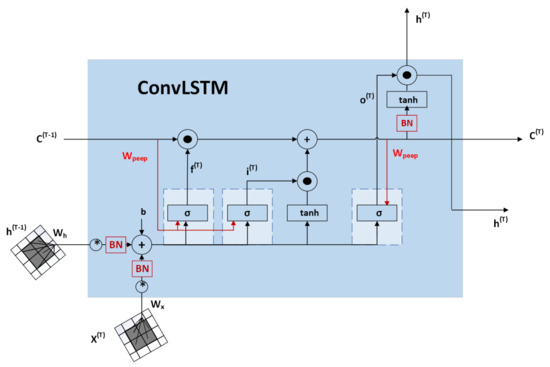
\includegraphics[width=0.8\textwidth]{figures/conv_lstm_architecture.jpg}
        \caption{A single ConvLSTM cell and its gated state transitions, adapted
        from Vrskova et al.~\cite{vrskova2022}.}
        \label{fig:convlstm-cell}
    \end{figure}

    Figure~\ref{fig:convlstm-cell} shows how one ConvLSTM cell combines the current
    spatial input $x_t$ with the previous hidden and cell states. Its gates control what
    information is retained in $C_t$ and exposed through $H_t$, preserving spatial
    structure while accumulating temporal context.

    At each time step $t$, the cell operations are defined as

    \begin{align}
        i_t &= \sigma\big(W_{xi} * x_t + W_{hi} * H_{t-1} + W_{ci} \circ C_{t-1} + b_i\big), \label{eq:input_gate} \\
        f_t &= \sigma\big(W_{xf} * x_t + W_{hf} * H_{t-1} + W_{cf} \circ C_{t-1} + b_f\big), \label{eq:forget_gate} \\
        C_t &= f_t \circ C_{t-1} + i_t \circ \tanh\big(W_{xc} * x_t + W_{hc} * H_{t-1} + b_c\big), \label{eq:cell_state} \\
        o_t &= \sigma\big(W_{xo} * x_t + W_{ho} * H_{t-1} + W_{co} \circ C_t + b_o\big), \label{eq:output_gate} \\
        H_t &= o_t \circ \tanh(C_t). \label{eq:hidden_state}
    \end{align}

    Here ``$*$'' denotes convolution, ``$\circ$'' the Hadamard product, and
    $\sigma(\cdot)$ the logistic sigmoid. The final hidden state $H_T$ summarizes the
    full clip.

    \subsubsection{Stage 3 --- Batch normalization}

    To stabilize the distribution of activations entering the next convolution, batch normalization is applied channel-wise over the mini-batch:

    \begin{equation}
        z = \gamma \cdot \frac{H_T - \mu}{\sqrt{\sigma^2 + \varepsilon}} + \beta,
        \label{eq:batchnorm}
    \end{equation}

    where $\mu$ and $\sigma^2$ are the batch mean and variance of $H_T$, and $\gamma, \beta$ are learned scale and shift parameters. This reduces internal covariate shift and, empirically, allows a higher learning rate without divergence.

    \subsubsection{Stage 4 --- Spatial feature refinement}

    A second 2-D convolution refines the normalized spatio-temporal feature map:

    \begin{equation}
        x' = \mathrm{ReLU}(W_r * z + b_r),
        \label{eq:stage4}
    \end{equation}

    followed by dropout, applied element-wise with rate $p$ during training:

    \begin{equation}
        x'' = m \circ x' / (1 - p), \qquad m_j \sim \mathrm{Bernoulli}(1 - p).
        \label{eq:dropout1}
    \end{equation}

    Inverted dropout scaling (division by $1-p$) keeps the expected activation magnitude unchanged at inference time, when no units are dropped.

    \subsubsection{Stage 5 --- Classification head}

    The refined feature map is flattened to a vector $v \in \R^{d}$ and passed through two fully connected layers:

    \begin{align}
        h &= \mathrm{Dropout}\big(\mathrm{ReLU}(W_1 v + b_1),\, p\big), \label{eq:fc1} \\
        \hat{y} &= \mathrm{softmax}(W_2 h + b_2), \qquad \hat{y} \in \R^{K}. \label{eq:softmax}
    \end{align}

    with the hidden layer set to 256 units, matching Algorithm~\ref{alg:convlstm}. The softmax output $\hat{y}$ is the estimated posterior over the $K$ activity classes, used both for prediction ($\hat{y}_{\mathrm{class}} = \arg\max_k \hat{y}_k$) and for the loss in Section~\ref{sec:training}.

    Relative to transformer or 3-D CNN alternatives, this architecture's convolutional--recurrent inductive bias constrains the hypothesis space it can represent. That constraint is intentional here: with the modestly sized surveillance datasets used in this study, it lets $\varphi$ and $g$ be learned reliably without large-scale pretraining, at the cost of the longer-range temporal modeling capacity that attention-based alternatives would offer on larger data.

    \begin{algorithm}[h]
        \caption{Proposed ConvLSTM Forward Pass}
        \label{alg:convlstm}
        \begin{algorithmic}[1]
            \Require Clip $V = (f_1, \ldots, f_T)$, $f_t \in \R^{H \times W \times C}$
            \Require Parameters $\theta = \{W_s, b_s,\ \text{ConvLSTM weights},\ \gamma, \beta,\ W_r, b_r,\ W_1, b_1,\ W_2, b_2\}$
            \Ensure Predicted class label $\hat{y}_{\mathrm{class}}$
            \For{$t = 1$ \textbf{to} $T$} \Comment{Stage 1: per-frame spatial encoding, Eq.~\eqref{eq:stage1}}
                \State $x_t \gets \mathrm{ReLU}(\mathrm{Conv2D}(f_t; W_s, b_s))$
            \EndFor
            \State $H_0, C_0 \gets 0, 0$
            \For{$t = 1$ \textbf{to} $T$} \Comment{Stage 2: ConvLSTM2D recurrence, Eqs.~\eqref{eq:input_gate}--\eqref{eq:hidden_state}}
                \State $i_t, f_t, o_t \gets \textsc{Gates}(x_t, H_{t-1}, C_{t-1})$
                \State $C_t \gets f_t \circ C_{t-1} + i_t \circ \tanh(\mathrm{Conv}(x_t, H_{t-1}))$
                \State $H_t \gets o_t \circ \tanh(C_t)$
            \EndFor
            \State $z \gets \mathrm{BatchNorm}(H_T; \gamma, \beta)$ \Comment{Stage 3, Eq.~\eqref{eq:batchnorm}}
            \State $x' \gets \mathrm{ReLU}(\mathrm{Conv2D}(z; W_r, b_r))$ \Comment{Stage 4, Eq.~\eqref{eq:stage4}}
            \State $x'' \gets \mathrm{Dropout}(x', p)$ \Comment{Eq.~\eqref{eq:dropout1}}
            \State $v \gets \mathrm{Flatten}(x'')$
            \State $h \gets \mathrm{Dropout}(\mathrm{ReLU}(W_1 v + b_1),\, p)$ \Comment{Stage 5, Eq.~\eqref{eq:fc1}}
            \State $\hat{y} \gets \mathrm{Softmax}(W_2 h + b_2)$ \Comment{Eq.~\eqref{eq:softmax}}
            \State $\hat{y}_{\mathrm{class}} \gets \arg\max_k \hat{y}[k]$
            \State \Return $\hat{y}_{\mathrm{class}}$
        \end{algorithmic}
    \end{algorithm}

    Lines 1--3 correspond to Stage 1 (Eq.~\eqref{eq:stage1}), lines 5--9 to Stage 2 (Eqs.~\eqref{eq:input_gate}--\eqref{eq:hidden_state}), line 10 to Stage 3 (Eq.~\eqref{eq:batchnorm}), lines 11--12 to Stage 4 (Eqs.~\eqref{eq:stage4}--\eqref{eq:dropout1}), and lines 13--16 to Stage 5 (Eqs.~\eqref{eq:fc1}--\eqref{eq:softmax}), giving a one-to-one correspondence between the algorithm and the equations defining $\varphi$ and $g$ in Section~\ref{sec:architecture}.

    \subsection{Training Procedure}
    \label{sec:training}

    The network is trained end-to-end in a supervised setting on labeled activity clips $\{(V^{(n)}, y^{(n)})\}_{n=1}^{N}$, where $y^{(n)}$ is a one-hot encoding of the ground-truth class over $K$ categories. The objective is the categorical cross-entropy loss

    \begin{equation}
        L_{CE}(\theta) = -\frac{1}{N} \sum_{n=1}^{N} \sum_{k=1}^{K} y_k^{(n)} \log \hat{y}_k^{(n)}(\theta),
        \label{eq:crossentropy}
    \end{equation}

    where $y_k^{(n)}$ is the $k$-th entry of the ground-truth one-hot vector for sample $n$, and $\hat{y}_k^{(n)}(\theta) = g(\varphi(V^{(n)}))_k$ is the corresponding predicted probability from Eq.~\eqref{eq:softmax}. This objective is well suited to multi-class classification because it penalizes low predicted probability mass on the true class more heavily as that probability approaches zero.

    To further discourage overfitting, an $L_2$ weight-decay term is added to the objective:

    \begin{equation}
        L(\theta) = L_{CE}(\theta) + \lambda \lVert \theta \rVert_2^2,
        \label{eq:regularized}
    \end{equation}

    with weight-decay coefficient $\lambda$ controlling the strength of the $L_2$ penalty on the network parameters $\theta$.

    Parameters are updated with Adam, which maintains exponential moving averages of the gradient (first moment) and its square (second moment) for adaptive, per-parameter step sizes:

    \begin{align}
        m_t &= \beta_1 m_{t-1} + (1-\beta_1) g_t, \qquad
        v_t = \beta_2 v_{t-1} + (1-\beta_2) g_t^2, \label{eq:adam1} \\
        \hat{m}_t &= \frac{m_t}{1-\beta_1^{t}}, \qquad
        \hat{v}_t = \frac{v_t}{1-\beta_2^{t}}, \label{eq:adam2} \\
        \theta_t &= \theta_{t-1} - \eta \frac{\hat{m}_t}{\sqrt{\hat{v}_t} + \varepsilon}, \label{eq:adam3}
    \end{align}

    where $g_t = \nabla_\theta L(\theta_{t-1})$ is the gradient at step $t$, $\eta$ is the learning rate, and $\beta_1, \beta_2$ control the decay rates of the moment estimates. Dropout (Eqs.~\eqref{eq:dropout1}, \eqref{eq:fc1}) is active only during this training procedure and is disabled at inference, when the model uses the full network deterministically.

    Together, Eqs.~\eqref{eq:crossentropy}--\eqref{eq:adam3} specify the complete optimization procedure: at each training step, a mini-batch of clips is forward-propagated through Algorithm~\ref{alg:convlstm} to obtain $\hat{y}$, the regularized loss~\eqref{eq:regularized} is computed, gradients are back-propagated through every stage of Section~\ref{sec:architecture}, and parameters are updated via the Adam rule~\eqref{eq:adam1}--\eqref{eq:adam3} until convergence.


    % =============================
    % Experimental Results and Discussion
    % =============================
    \section{Experimental Results and Discussion}
    \label{sec:results}

    This section evaluates how ConvLSTM depth, width, and temporal input affect abnormal activity
    recognition. The architecture search is first used to identify compact, high-performing ConvLSTM
    configurations, after which the selected models are compared with representative ConvLSTM, 3D
    CNN, and transformer-based architectures. The overall objective is to identify a lightweight
    ConvLSTM configuration that maintains strong classification performance with substantially
    fewer trainable parameters.

    \subsection{Experimental Setup}
    \label{sec:experimental-setup}

    The Abnormal Activities Dataset (AAD)~\cite{vrskova2022} contains 1,069 video clips across 11
    classes: Begging, Drunkenness, Fight, Harassment, Hijack, Knife Hazard, Normal Videos, 
    Pollution, Property Damage, Robbery, and Terrorism. The dataset contains scenes recorded under
    different lighting conditions, camera viewpoints, object positions, and environments, including
    buildings, parking areas, and outdoor locations. These variations make the dataset suitable for
    evaluating abnormal human activity recognition under diverse visual conditions.

    The experiments were conducted using Google Colab with an NVIDIA A100-SXM4 GPU with 80~GB of 
    memory, PyTorch 2.9.1+cu128, and CUDA 12.8.

    The architecture search was designed to identify a compact ConvLSTM configuration that performs
    consistently across different temporal input settings. A configuration such as
    \texttt{ConvLSTM[64,64,128]} represents three stacked ConvLSTM layers with 64, 64, and 128 
    filters, respectively. This notation allows both the number of recurrent layers and the width
    of each layer to be varied.

    A total of 32 candidate architectures were evaluated, covering one to five ConvLSTM layers
    with widths ranging from 16 to 128 filters. The search included flat, expanding, contracting,
    and middle-wide configurations, while all spatial kernels were fixed at $3\times3$. Each
    architecture was evaluated at $32\times32$ resolution under four temporal conditions: 8 or 16
    frames sampled at either 8 or 16~FPS, this produced a total of 128 architecture search runs.

    Input frames were sampled at fixed target timestamps from the beginning of each video, resized,
    and normalized to $[0,1]$.Short clips were padded by repeating the final available frame, 
    whereas longer clips were sampled only within the fixed temporal window used as model input.

    All ConvLSTM search models were trained using Adam with a batch size of 32, no data 
    augmentation, zero weight decay, and a validation-loss \texttt{ReduceLROnPlateau} scheduler
    with factor 0.9 and patience of 5 epochs. Search and resolution check runs used a maximum of
    128 epochs, a minimum training length of 64 epochs, and early-stopping patience of 16 epochs.
    The final comparison runs used a maximum of 256 epochs, a minimum of 64 epochs, and 
    early-stopping patience of 32 epochs.

    The dataset was divided into 70\% training, 15\% validation, and 15\% testing subsets using
    a stratified split to preserve class proportions. The initial learning rate was $10^{-3}$
    for all models.
    
    \subsection{Architecture-Search Results}
    \label{sec:search-results}

    Figure~\ref{fig:aad_search_capacity} shows validation accuracy as a function of trainable
    parameter count for all 128 architecture search runs. Models were ranked using mean
    validation accuracy across the four temporal conditions, followed by worst-case validation
    accuracy, mean validation loss, parameter count, and model name. This ranking reduces the
    influence of a single favourable input configuration when selecting candidates.

    \begin{figure}[!htbp]
        \centering
        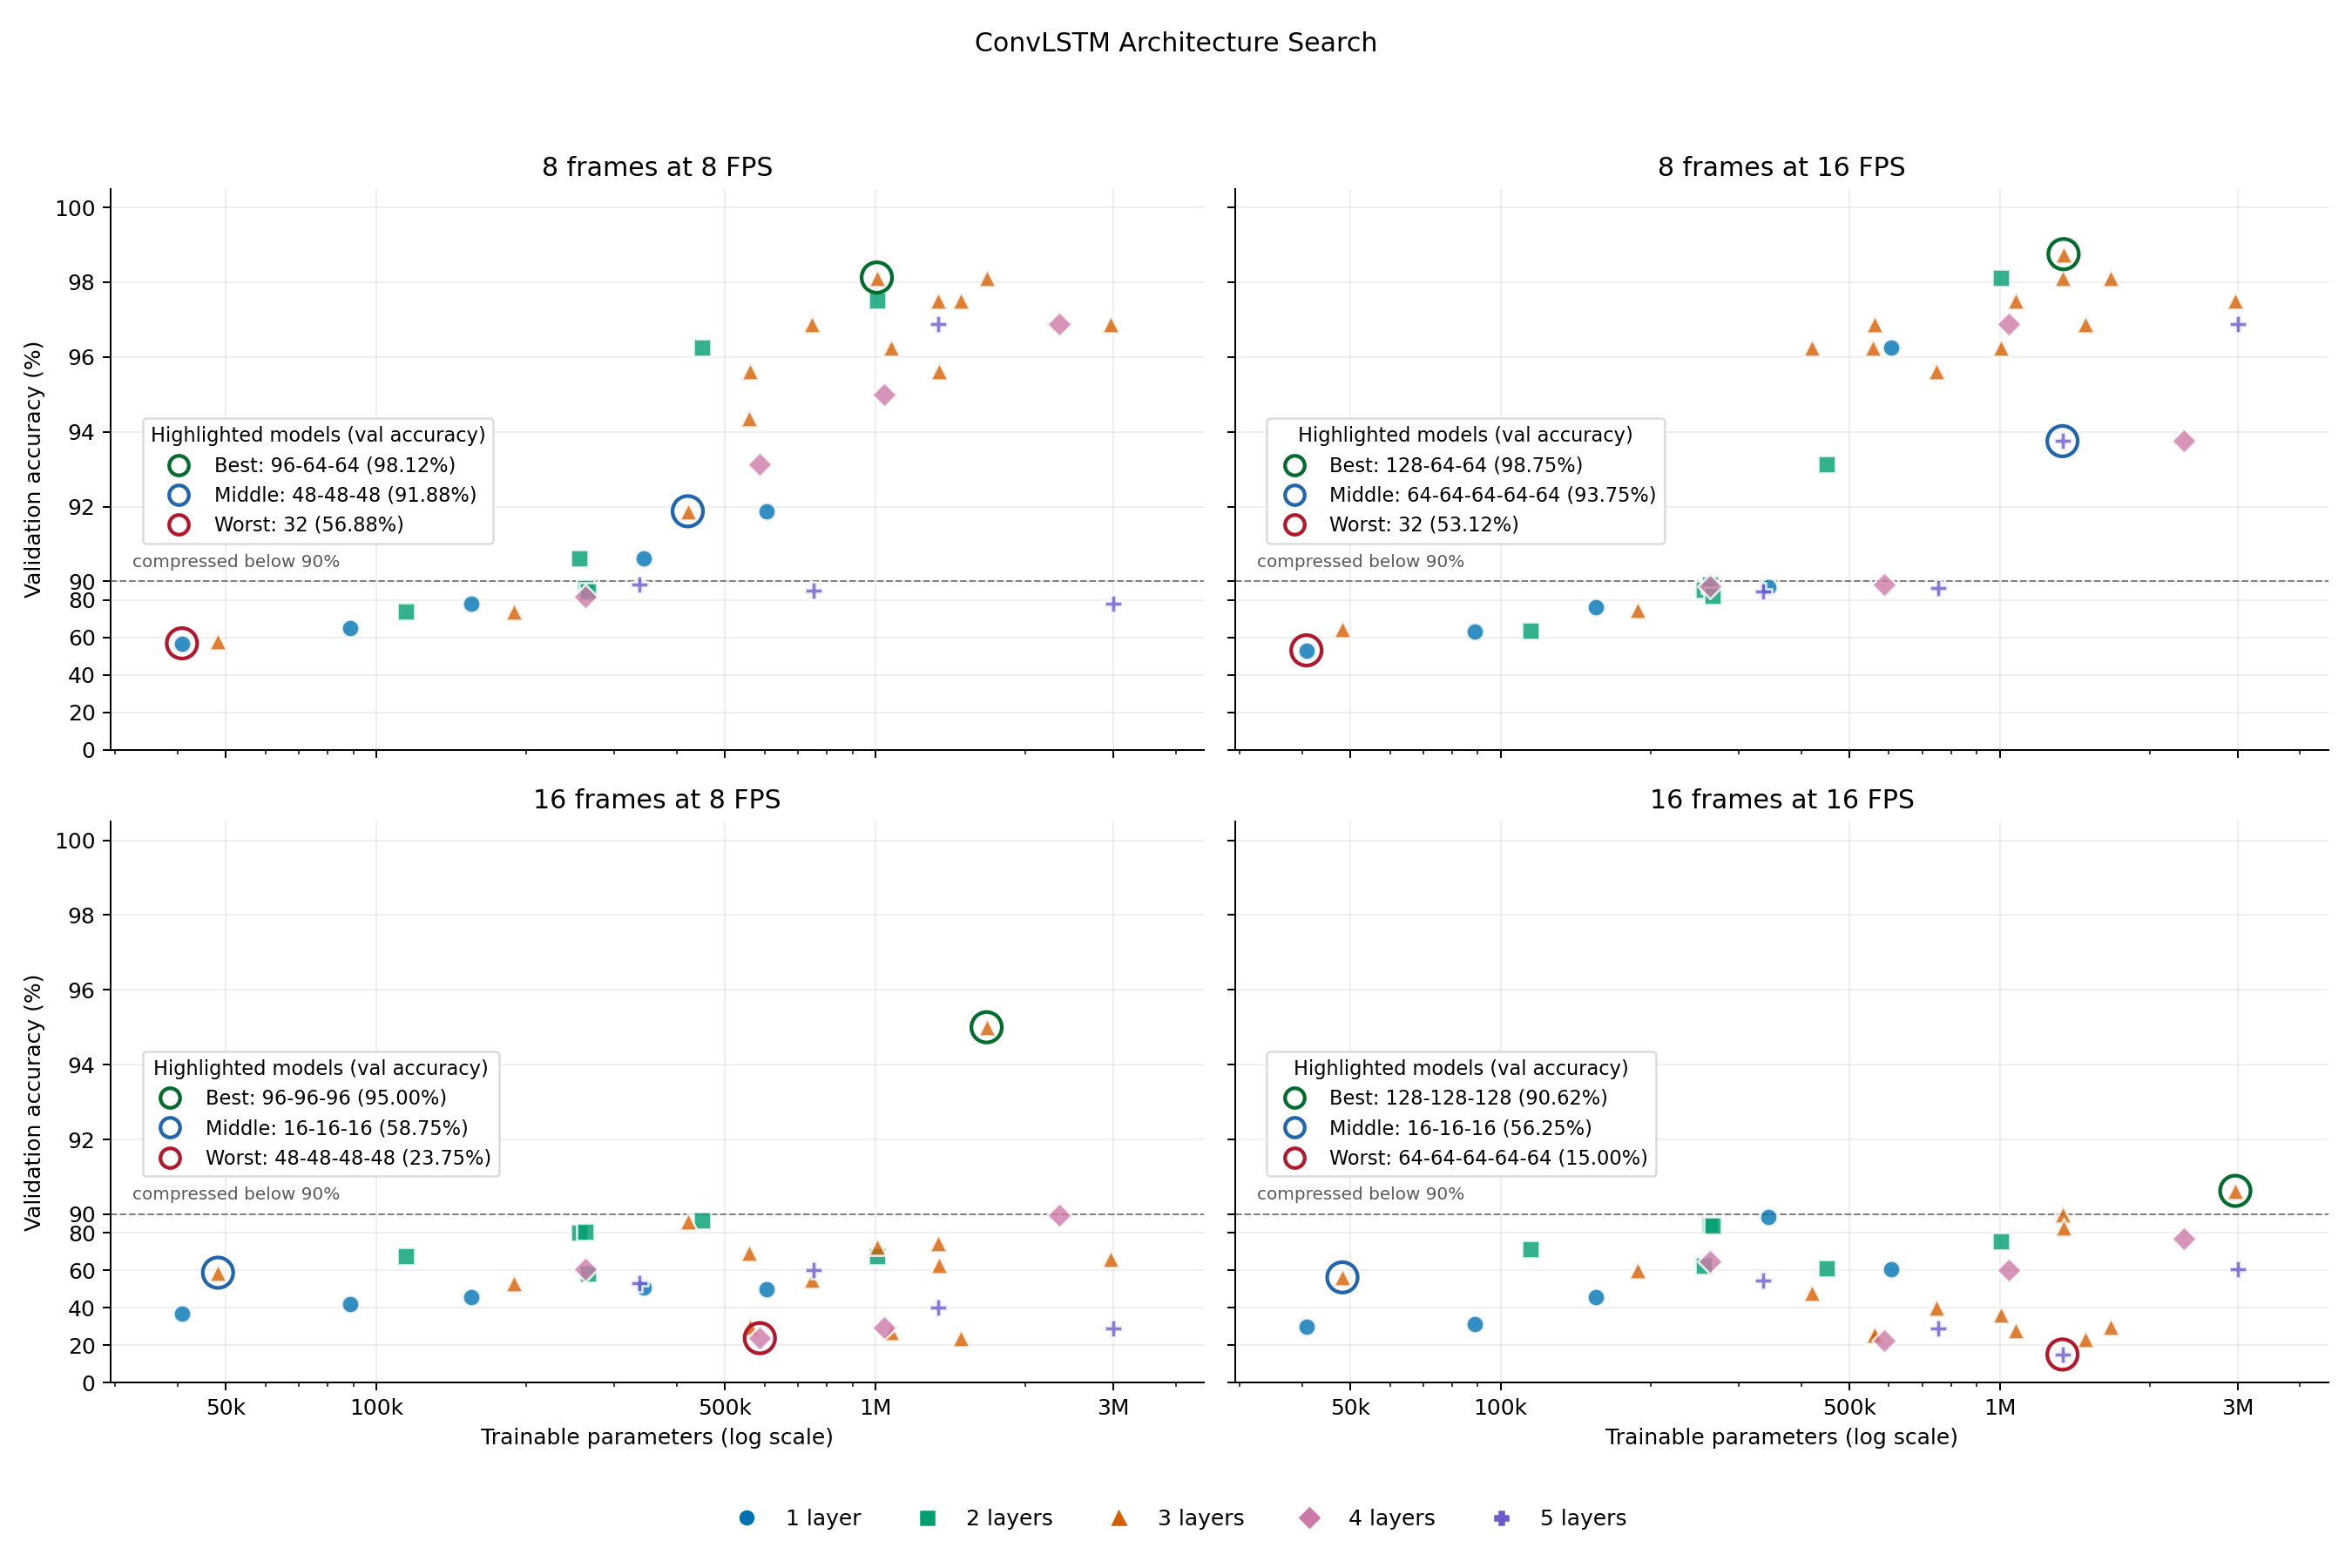
\includegraphics[width=\textwidth]{figures/2026-10-16/search_capacity.png}
        \caption{Validation accuracy versus parameter count for the ConvLSTM architecture
        search. Colours and markers indicate recurrent depth, while rings identify selected
        high, middle, and low performing observations within each panel. Parameter count is
        shown on a logarithmic scale.}
        \label{fig:aad_search_capacity}
    \end{figure}

    The temporal configuration had a substantial effect on performance, for example, the 
    eight-frame inputs, the mean validation accuracy across the 32 architectures was 88.03\%
    at 8~FPS and 88.18\% at 16~FPS. Increasing the sequence length to 16 frames reduced these
    means to 57.03\% and 53.57\%, respectively. Training accuracy followed the same trend,
    decreasing from approximately 92\% to 61\% and 57\%. Longer sequences therefore did not
    improve performance within the available training budget. Since both training and
    validation performance decreased, this behaviour is more consistent with optimization
    difficulty or increased temporal complexity than with conventional overfitting. 
    Furthermore, 108 of the 128 runs reached the epoch limit.

    Figure~\ref{fig:aad_capacity_controls} separates the effects of model depth and width.
    At a width of 96 filters, average validation accuracy increased up to four ConvLSTM layers,
    reaching 89.219\%, before falling to 66.094\% at five layers. In contrast, within the
    three layers width sweep, the widest tested configuration, \texttt{ConvLSTM[128,128,128]},
    remained the strongest. These results indicate that increasing capacity can improve
    performance, but the benefit depends on how that capacity is distributed across the
    architecture.

    \begin{figure}[!htbp]
        \centering
        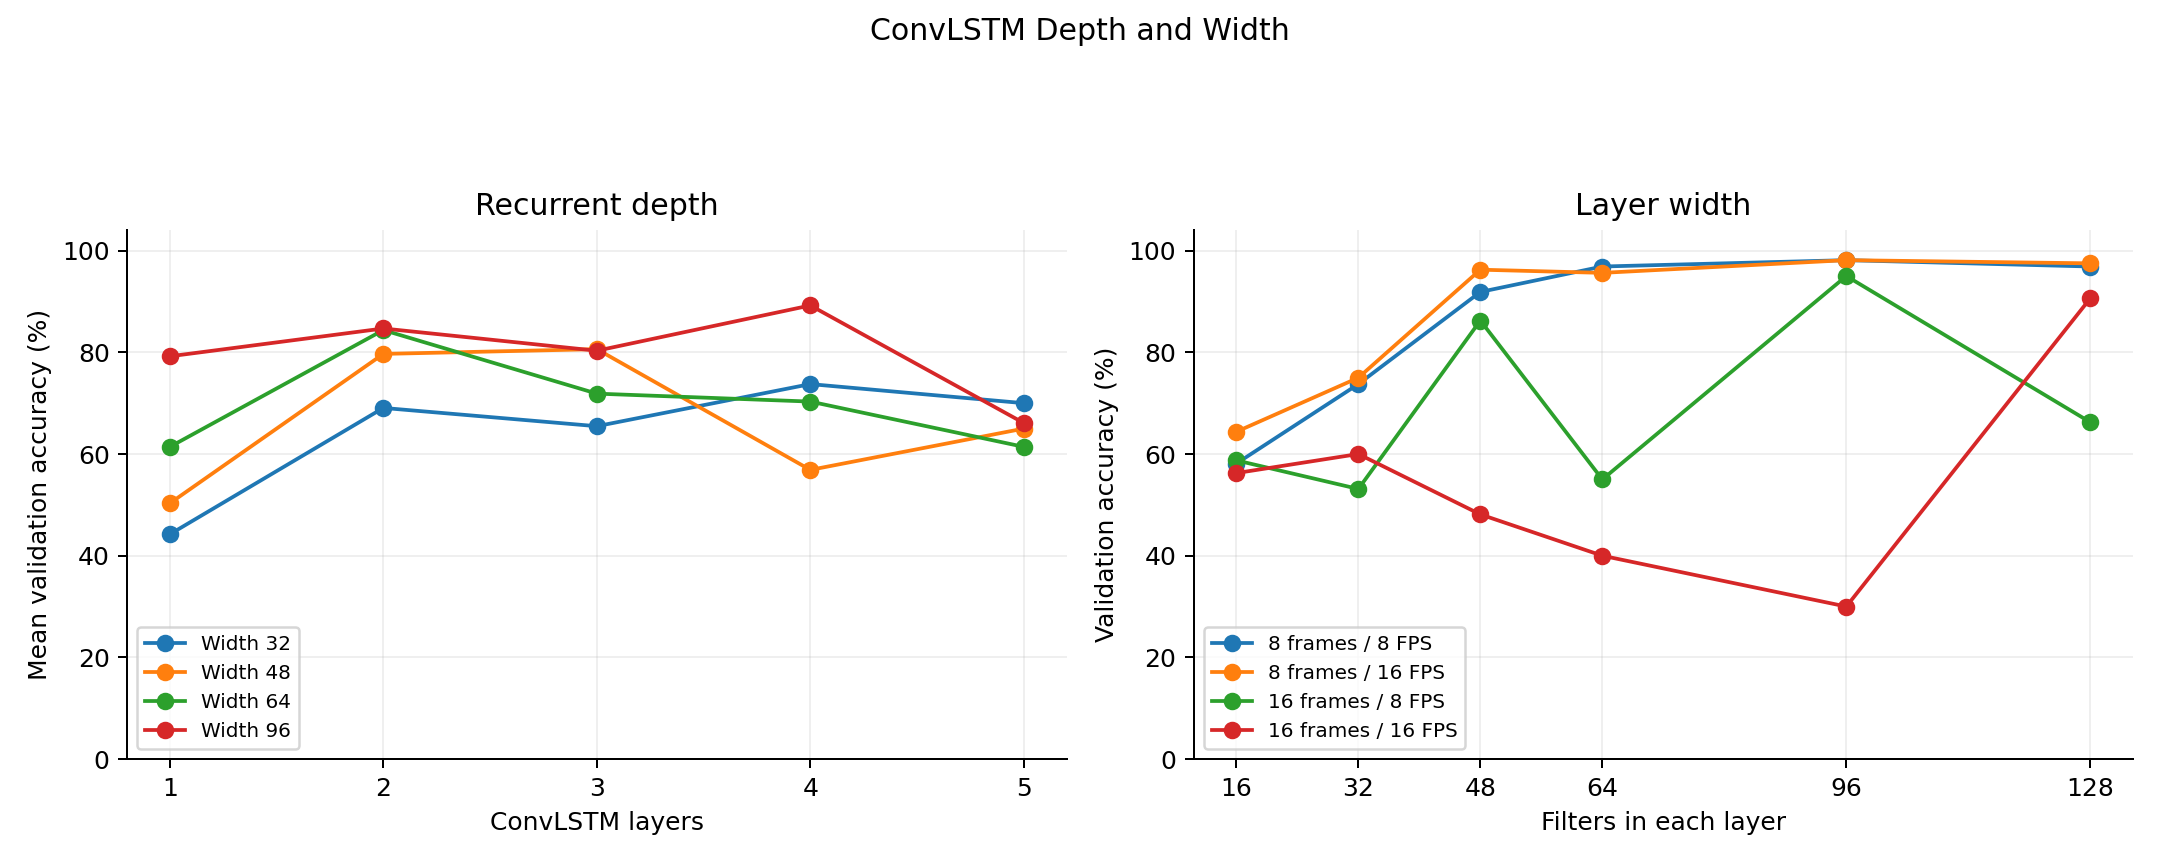
\includegraphics[width=\textwidth]{figures/2026-10-16/capacity_controls.png}
        \caption{Effects of ConvLSTM depth and width on validation accuracy. Left: flat-stack
        depth comparisons averaged across the four temporal conditions. Right: three-layer
        width comparisons separated by temporal condition. Both panels are derived from the
        same architecture search.}
        \label{fig:aad_capacity_controls}
    \end{figure}

    Filter placement also influenced the observed performance. The four-condition mean
    accuracy was 71.875\% for \texttt{ConvLSTM[64,64,64]}, 85.156\% when the first layer was
    widened to 128 filters, 60.313\% when the middle layer was widened, and 90.000\% when
    the final layer was widened. The \texttt{ConvLSTM[64,64,128]} configuration therefore
    provided a strong balance by maintaining moderate early-layer capacity while expanding
    the final representation. However, because these configurations also differ in parameter
    count, the effect cannot be attributed to filter placement alone.

    The five highest ranked architectures were selected for the final comparison. Across
    these finalists, eight frames sampled at 16~FPS produced the highest mean validation
    accuracy, reaching 95.250\%, compared with 94.625\% at 8~FPS. The finalists were then
    evaluated at $64\times64$ resolution before final training.

    \clearpage
    \subsection{Comparative Evaluation}
    \label{sec:aad-comparison}

    The five selected ConvLSTM configurations were compared with the input-adapted
    ConvLSTM of Vršková et al.~\cite{vrskova2022}, the R3D-18 and MC3-18 architectures of
    Tran et al.~\cite{tran2018closer}, and the Swin3D-T and Swin3D-S video transformers of
    Liu et al.~\cite{liu2022videoswin}.

    All reference models were retrained from scratch on AAD using the same train,
    validation, and test split and the same input of eight $64\times64$ frames sampled at
    16~FPS. Training followed the procedure described in 
    Section~\ref{sec:experimental-setup}.

    Final training ran for 256 epochs and each model retained the checkpoint with the
    lowest validation loss, and the final ConvLSTM configuration was selected using
    validation accuracy, followed by validation loss and parameter count. The test set
    was evaluated only after all model-selection decisions had been frozen.

    Classification performance was measured using accuracy, macro-averaged precision,
    recall, and F1-score. Accuracy is defined as

    \begin{equation}
        \mathrm{Accuracy}=\frac{1}{N}\sum_{n=1}^{N}
        \mathbf{1}\!\left[\hat{y}_n=y_n\right].
        \label{eq:accuracy}
    \end{equation}

    For each class $c$, let $TP_c$, $FP_c$, and $FN_c$ denote the true-positive, 
    false-positive, and false-negative counts. Macro precision, recall, and 
    F1-score are then

    \begin{align}
        \mathrm{Precision}&=\frac{1}{K}\sum_{c=1}^{K}
            \frac{TP_c}{TP_c+FP_c}, \label{eq:precision}\\
        \mathrm{Recall}&=\frac{1}{K}\sum_{c=1}^{K}
            \frac{TP_c}{TP_c+FN_c}, \label{eq:recall}\\
        \mathrm{F1}&=\frac{1}{K}\sum_{c=1}^{K}
            \frac{2TP_c}{2TP_c+FP_c+FN_c}. \label{eq:f1}
    \end{align}

    where $K=11$. Undefined class scores were assigned zero. Test loss is
    reported as mean cross-entropy loss, while parameter count includes all
    learnable weights and biases.

    \begin{table}[!htbp]
        \centering
        \small
        \setlength{\tabcolsep}{4pt}
        \caption{Test performance of the selected ConvLSTM configurations
        and retrained reference models on AAD.}
        \label{tab:aad_results}
        \resizebox{\textwidth}{!}{%
            \begin{tabular}{@{}lrrrrrr@{}}
                \toprule
                Model & Acc (\%) & Prec (\%) & Rec (\%) & F1 (\%) & 
                Parameters & Loss\\
                \midrule
                \texttt{ConvLSTM[64,64,128]}    & \textbf{99.379} & 
                \textbf{99.242} & \textbf{99.174} & \textbf{99.172} 
                & 1,336,459 & \textbf{0.0403}\\
                \texttt{ConvLSTM[96,96,96,96]}  & 98.137 & 98.331 & 
                97.989 & 98.092 & 2,335,403 & 0.0798\\
                \texttt{ConvLSTM[128,128,128]}  & 98.758 & 98.737 & 
                98.669 & 98.652 & 2,965,899 & 0.0513\\
                \texttt{ConvLSTM[128,64,64]}    & 98.137 & 98.158 & 
                98.033 & 98.024 & 1,342,667 & 0.0938\\
                \texttt{ConvLSTM[32,64]}        & 92.547 & 93.802 & 
                92.119 & 92.476 & \textbf{262,603} & 0.3068\\
                \midrule
                Vrskova et al.~\cite{vrskova2022} (adopted) & 94.410 & 
                95.306 & 94.216 & 94.510 & 134,415,195 & 0.7242\\
                Tran et al.~\cite{tran2018closer} (3D)     & 95.031 & 
                95.724 & 95.827 & 95.680 & 33,171,915 & 0.1661\\
                Tran et al.~\cite{tran2018closer} (mixed)  & 97.516 & 
                97.955 & 98.021 & 97.869 & 11,495,883 & 0.0695\\
                Liu et al.~\cite{liu2022videoswin} (tiny)  & 93.168 & 
                93.794 & 94.139 & 93.862 & 27,858,929 & 0.1496\\
                Liu et al.~\cite{liu2022videoswin} (small) & 95.031 & 
                95.595 & 95.662 & 95.561 & 49,517,537 & 0.1437\\
                \bottomrule
            \end{tabular}%
        }
        \par\smallskip
        \begin{minipage}{\textwidth}
            \footnotesize Precision, recall, and F1 are macro-averaged across all 11
            classes as defined in Eqs.~\eqref{eq:precision}--\eqref{eq:f1}
        \end{minipage}
    \end{table}

    Table~\ref{tab:aad_results} shows that \texttt{ConvLSTM[64,64,128]} achieved the
    highest observed test accuracy of 99.379\% using 1,336,459 parameters. The smallest
    finalist, \texttt{ConvLSTM[32,64]}, reduced the parameter count further to 262,603,
    but its accuracy decreased to 92.547\%. These results indicate that aggressive
    parameter reduction eventually degrades performance, while the selected three layers
    configuration provides a stronger accuracy--complexity trade-off.

    \subsection{Discussion and Confusion Analysis}
    \label{sec:aad-discussion}

    The proposed architecture does not introduce a new recurrent memory mechanism, its
    contribution lies in how ConvLSTM layers and the classification head are arranged.
    The adapted Vršková~\cite{vrskova2022} architecture applies a frame-level convolution,
    a single ConvLSTM layer, a post-convolution, and a large flattened dense classifier.
    In contrast, the proposed family stacks configurable ConvLSTM layers and applies
    global spatial pooling before a lightweight classification head. This design
    substantially reduces the parameter count, with much of the reduction resulting from
    removal of the large flattened classifier.

    The architecture search further showed that the distribution of recurrent capacity
    matters. In particular, the selected \texttt{ConvLSTM[64,64,128]} configuration
    preserves moderate width in the first two layers and expands the final representation.
    It consistently performed well compared with flat and middle-wide alternatives.

    For the selected model, the confusion matrix is defined as

    \begin{equation}
        C_{ij}=\sum_{n=1}^{N}
        \mathbf{1}\!\left[y_n=i\right]
        \mathbf{1}\!\left[\hat{y}_n=j\right],
        \qquad i,j\in\{1,\ldots,K\}.
        \label{eq:confusion-matrix}
    \end{equation}

    Rows represent the true classes and columns the predicted classes. Diagonal entries
    correspond to correct classifications, while off-diagonal entries represent
    classification errors.

    Figure~\ref{fig:cm_aad} shows that the selected model correctly classified 160 of
    the 161 test clips. The only error occurred when a Hijack clip was classified as
    Terrorism, resulting in a Hijack recall of 90.91\% and a Terrorism precision of
    91.67\%. The remaining nine classes achieved perfect observed precision, recall,
    and F1-score.

    \begin{figure}[!htbp]
        \centering
        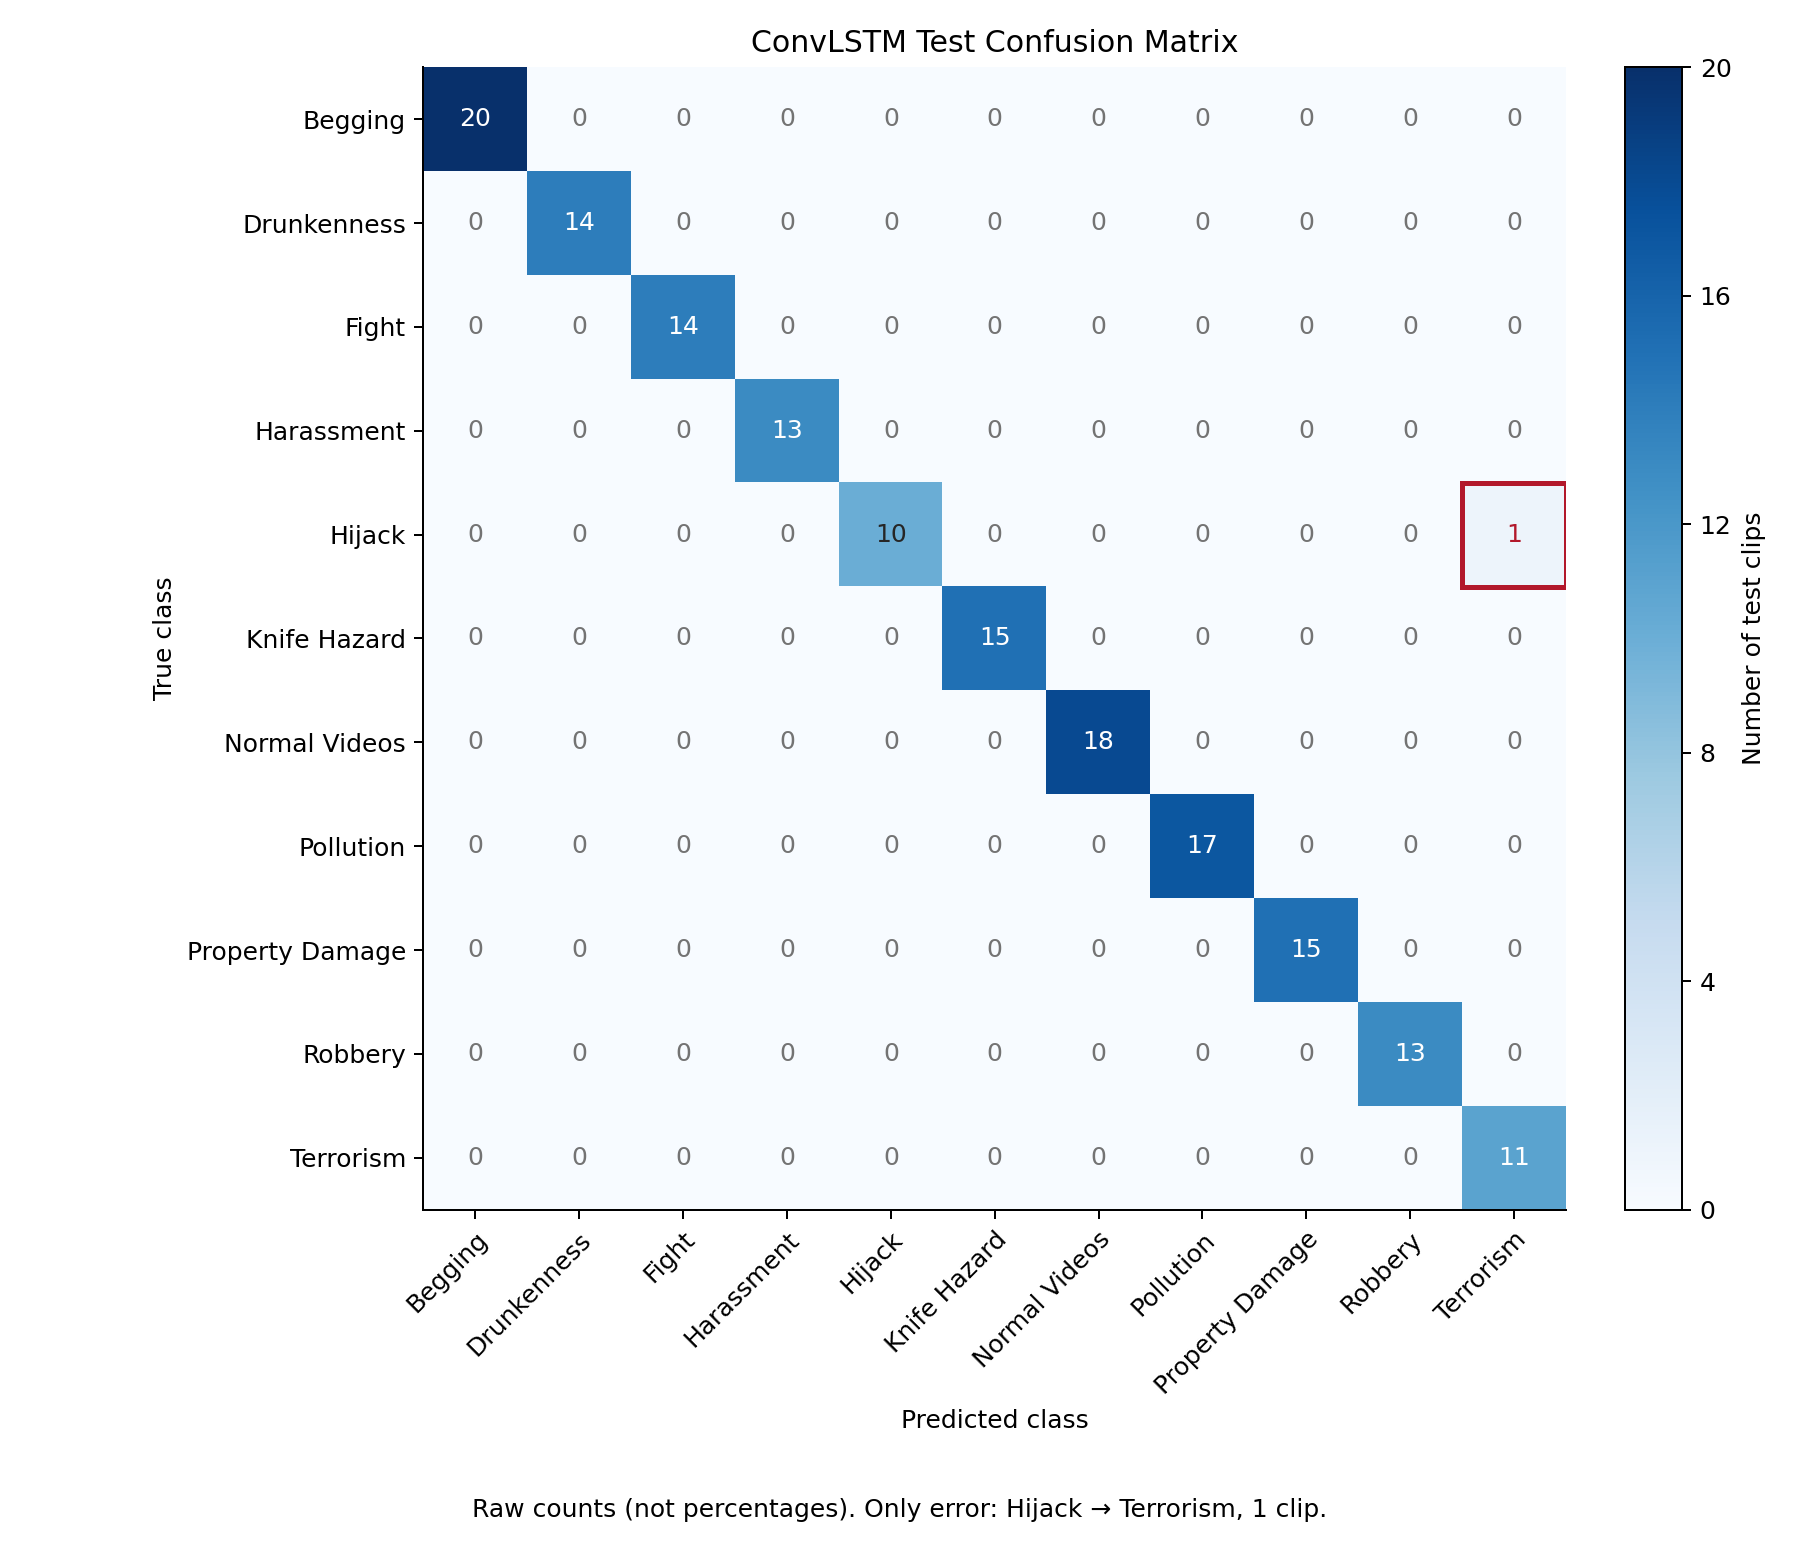
\includegraphics[width=0.88\textwidth]{
            figures/2026-10-16/best_model_test_confusion.png}
        \caption{Test confusion matrix of the validation-selected
        \texttt{ConvLSTM[64,64,128]} model. Entries are raw clip counts, rows
        represent true classes and columns represent predicted classes.}
        \label{fig:cm_aad}
    \end{figure}

    The reduced parameter count makes the proposed architecture attractive for
    resource constrained applications because it lowers model-storage requirements
    and the global pooling classifier does not grow with frame resolution or sequence
    length. However, parameter count alone does not determine inference speed. ConvLSTM
    computation and recurrent-state memory still increase with spatial and temporal
    input size. The present results therefore demonstrate parameter efficiency rather
    than real-time or edge-deployment performance.

    Finally, the selected input of eight frames at 16~FPS spans only 0.4375 seconds
    from the first to the last sampled frame. Events outside this temporal window may
    therefore be missed. The current model also assigns a single label to each clip
    and does not preserve recurrent state across consecutive windows. Future work should
    investigate longer-duration modelling, multi-label activity recognition, 
    independent scene evaluation, repeated-seed experiments, and direct inference time
    measurements.

    \clearpage
	% =============================
	% Conclusion and Future Work
	% =============================
	\section{Conclusion and Future Work}
	\label{sec:conclusion}

	This paper presented a lightweight ConvLSTM architecture for abnormal human activity 
	recognition in surveillance video. Following an empirical capacity search from the 
	original 4M parameter baseline~\cite{vrskova2022}, the proposed Custom 
	(64-32-16-64) configuration achieves 96.74\% accuracy on the 11-class LoDVP dataset 
	and 88.57\% on the binary AIRTLab violence detection benchmark, matching or exceeding 
	both the original ConvLSTM baseline and standard 3D CNN architectures at 1.28M 
	parameters a 3.8$\times$ reduction. The combination of spatial augmentation, weight 
	decay, learning rate scheduling, and cross-dataset fine-tuning proved effective in 
	addressing the overfitting challenge posed by small surveillance datasets.

	Error analysis revealed that a subset of misclassifications occur between visually 
	similar classes such as Fight and Harassment, suggesting that some surveillance clips 
	inherently contain overlapping behavioural cues from multiple categories. This points 
	toward multi-label classification as a more appropriate formulation, where a clip is 
	not forced into a single hard class assignment. Additionally, the current model operates 
	on fixed-length short clips and does not retain context across clip boundaries,
	incorporating long-term temporal memory through hierarchical recurrence or memory-augmented 
	networks could improve recognition of activities that unfold over extended durations. 
	Future work will explore attention-based temporal localisation, multi-label reformulation, 
	and evaluation on the larger UCF-Crime benchmark to further validate generalisation to 
	real-world surveillance conditions.

	% =============================
	% References
	% =============================

	\bibliographystyle{IEEEtran}
	\bibliography{references}

\end{document}
